\section{Design}
\subsection{Objectives}
The main purpose of this research is to develop an approach to quickly training a robot to navigate successfully. To this end we will define the objectives of our research as follows.
\begin{enumerate}
	\item The algorithm should be capable of training a neural network to navigate an autonomous robot.
	\item The algorithm will be able to successfully train the robot in a quick and efficient manner. 
	\begin{enumerate}
		\item Where successfully train means to to be able to accomplish the retrieval task in a safe manner, meaning it does not collide with anything in the environment. Also meaning as to be able to accomplish it's task in an expedient manner. i.e. complete its task without unnecessary movements or stopping.
		\item And quick and efficient meaning a successful candidate neural network being produced within an acceptable number of generations. 
	\end{enumerate}
	\item The algorithm should be portable. Meaning the algorithm should not just be able to train for one type of robot. For example, the algorithm should be able to train on robots with reversible tracks, four wheels, etc.
\end{enumerate}

\subsection{IOANNIS Algorithm structure}
For training the neural network, a genetic algorithm was selected. This is because with a task such as navigation, it is hard to use back propagation for training, as that would require for each decision, the actual correct decision to be determined and then re-train the network. When using a genetic algorithm to train a fitness function can be defined, this can evaluate the performance of the algorithm, and then whichever weights work better towards the defined goals will be kept on to further improve the robot. 

The stages of the algorithm can be seen in figure \ref{fig:algorithmSteps} and can be summarised as follows.
\begin{enumerate}
	\item Produce an initial population of weights.
	\item For each set of weights in the population initialise a neural network using those weights and use it to operate the simulated robot. 
	\item Score the simulated robots and provide feedback to the genetic algorithm.
	\item Using feedback from the simulation the genetic algorithm will use its fitness function to rank each set of weights. 
	\item If the end condition is met, return the fittest set of weights. 
	\item Otherwise crossover or mutate the weights according to the crossover and mutations rates.
	\item Return to item 2 and repeat the process with the new population
\end{enumerate}

\begin{figure}[h]
	\begin{center}
		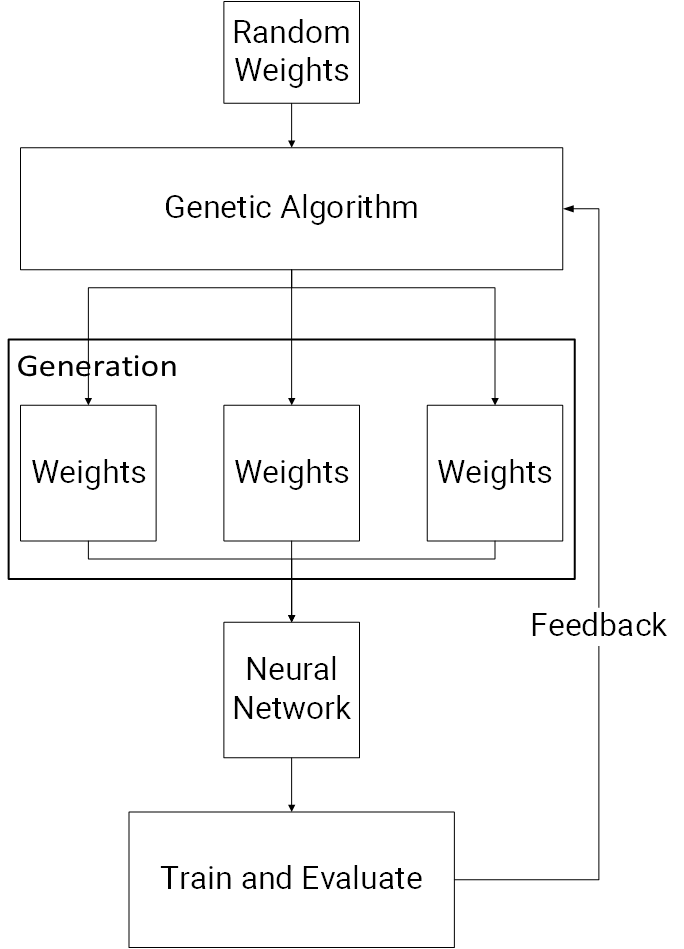
\includegraphics[width=0.75\linewidth]{steps}
		\caption{Stages of the IOANNIS algorithm}
		\label{fig:algorithmSteps}
	\end{center}
\end{figure}

The following sections will outline the design of the neural network and genetic algorithm that will train it. 

\subsection{Neural Network Design}
The neural network will use $l$ layers an input layer $I$ and output layer $O$ and $x$ hidden layers $H_x$. The weights for each node $W_{li}$, where $l$ represents the layer and $i$ represents the weight's index, will be populated and trained using a genetic algorithm described in section \ref{sec:GADesign} below.

\begin{figure}[h]
	\begin{center}
		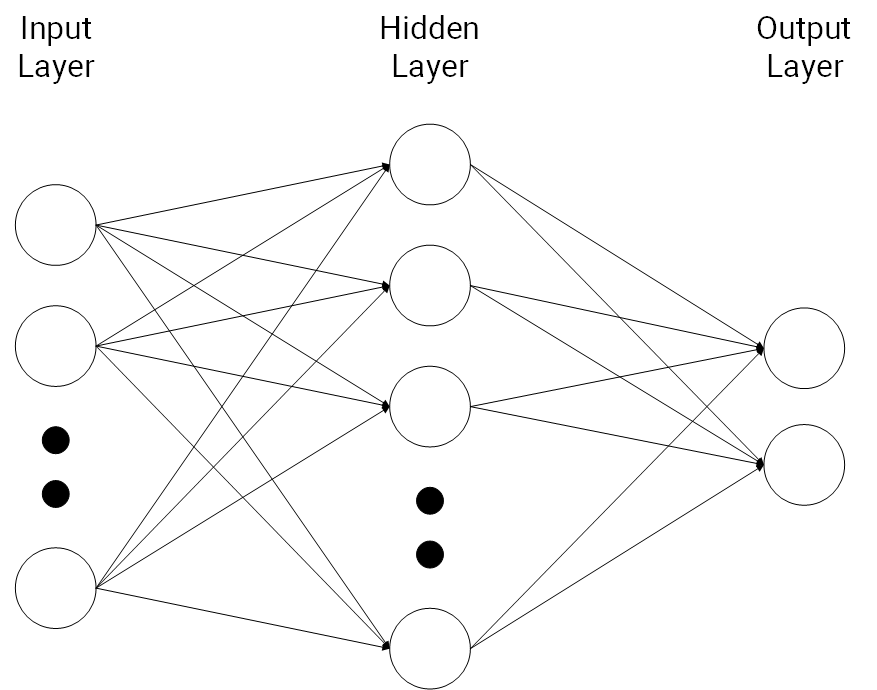
\includegraphics[width=1\linewidth]{nn}
		\caption{Representative Neural Network}
		\label{fig:neuralNetwork}
	\end{center}
\end{figure}

%For this task it has been elected to use an input layer consisting of $x$ nodes, one for each sensor input to the robot. We have then selected to use $y$ hidden layers of $z$ nodes, this is because of....

There will be two output nodes. Each output will have applied to it a tan-sigmoid transfer function (figure \ref{fig:tansig}) to smooth the output. We have selected the tan-sigmoid transfer function as one output will represent each track, with a positive output directing the track to run forward, and a negative output directing the track to run backwards. The magnitude of each output will be used to control the speed at which the track runs.

\begin{figure}[h]
	\begin{center}
		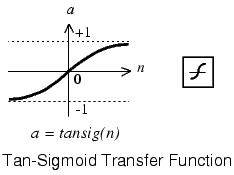
\includegraphics[width=0.5\linewidth]{tansig}
		\caption{Tan-Sigmoid Transfer Function}
		\label{fig:tansig}
	\end{center}
\end{figure}

\subsection{Genetic Algorithm Design}
\label{sec:GADesign}
The genetic algorithm will be used to hone the weights used by the neural network described above. 
\subsubsection{Genetic Operators}
Due to the nature of this task, we have elected to use three genetic operators. We have selected the three operators below, as due to the nature of this task, there is no need to use the operators for coercion where there are restrictions placed on an individuals viability. All candidates produces will be viable.
\begin{enumerate}
	\item \textit{Crossover Operator:} This will select another individual from the population and split it at a randomly selected point. The first section of genome A will be combined with the second section of genome B, and the first section of genome B will be combined with the second section of genome A. This will produce two children to be passed to the next generation.
	\item \textit{Mutation Operator:} This will randomly select a weight in the individual's genome, and randomly assign it a new weight between 0.00 and 1.00. The resulting child will then be passed into the next generation
	\item \textit{Pass-through Operator:} This operator will pass the selected individual directly through to the next generation without change. This is the default operator and will be selected if the other two are not.
\end{enumerate}

Each operator will have a chance of being selected proportional to it's selection probability.
\subsubsection{Fitness Function}
The fitness function to evaluate the fitness of an individual $f(I)$ shall be defined as follows.
\begin{equation}
	f(I) = c + t\label{eq:fitnessFunction}
\end{equation}
Where $c$ represents the number of collisions the robot makes, and $t$ represents the time it takes to complete it's task.
\subsubsection{End Condition}
To determine when the optimal solution has been found, there are two options. Firstly, it is possible to limit to a fixed number of generations, after which the fittest individual will be presented as the optimal solution. The other is to define an end condition, for this algorithm that could be defined as having an adaptable number of generations with at least one genome resulting in no collisions.

For the purpose this algorithm has been produced for, it is pertinent that the selected outcome prioritises safety of the robot and it's surroundings, as such the proposed algorithm will used a goal based end condition, and not be limited by the number of generations. This is because if a genome leads to collisions, this would be undesirable and unfit for purpose.